% =========================================================================
% CHAPTER 6 — THE ANALYTICAL PIPELINE (~2000 words body text)
% =========================================================================

\chapter{The Machine Learning Substrate}
\label{ch:data_pipeline}

\noindent
{\rmfamily\itshape
\begin{tabular}[t]{@{}l@{\hspace{0.3cm}}p{12.5cm}@{}}
\textls[50]{\textbf{Addressed:}} &
\textls[50]{Latent Structure · Dimensionality Reduction · Manifold Geometry · Early Warning
Signals · Pseudo-Replication \& Null Results · Anomaly Detection · Observation vs Reanalysis}
\end{tabular}
}

\vspace{0.5cm}

This chapter is the core of the \emph{detect} phase: the analysis that recovers, from the AMOC observational record, the latent structure the \emph{translate} phase will later make perceptible. It delivers objectives O1.1--O1.3 and tests the analytical hypotheses H1--H3. The aim is not a new claim about the ocean --- a reader looking for an oceanographic discovery will not find one here, and that is by design. It is narrower and, for this thesis, more important: to establish with evidence that the AMOC's vertical structure reduces to a small, faithful, interpretable set of coordinates, because everything the representation does in Chapter~\ref{ch:translate} rests on that substrate being trustworthy. The results are therefore framed by their implications for the representation rather than by their oceanographic significance.

The material is the RAPID-MOCHA-WBTS record at \ang{26.5}~north: the overturning streamfunction sampled at 307 depth levels over the period April 2004 to March 2024. Incomplete records near the end of the series are dropped, which leaves 14{,}596 profiles, each a vector of 307 numbers describing how the transport is distributed with depth.\footnote{The depth grid is close to uniform (spacing 19.33--19.87~m, median 19.59~m; a max/min ratio of 1.03), so no layer-thickness weighting is applied: with levels this evenly spaced, weighting would scale every level by an almost identical constant, which PCA absorbs without any effect on the loadings or the variance shares.} Before anything else, each profile is centred on the record mean, so the analysis describes how the vertical structure \emph{departs} from its average shape rather than simply recovering that average shape again.

% -------------------------------------------------------------------------
\section{Latent Structure \& PCA Decomposition}
\label{sec:detect-pca}
 
The first objective (O1.1) is to find the dominant modes of the AMOC's vertical variability using principal component analysis. The result is clear-cut: the variability is almost one-dimensional. A single mode accounts for \SI{89.82}{\percent} of the total variance in the vertical structure, and two modes together account for \SI{97.86}{\percent} (Table~\ref{tab:pca-variance}). From the third mode on, each mode adds less than \SI{1.6}{\percent}, and the scree curve bends sharply between the second and third modes --- the familiar elbow that marks where structure ends and noise begins. This confirms H1, and by a wide margin: the hypothesis expected two or three modes above \SI{80}{\percent} (\S\ref{sec:hypotheses}), and the data give two modes above \SI{97}{\percent}.
 
% figures/data_pipeline/tab_pca_variance.tex — variance explained by the PCA modes
% Numbers verified against NB03. Requires \usepackage{booktabs}.
\begin{table}[!ht]
    \centering
    \small
    \caption[Variance explained by the vertical PCA modes.]{Variance explained
    by each principal component of the AMOC vertical profiles. Two modes reach
    \SI{97.86}{\percent}; the tail beyond PC2 is noise.}
    \label{tab:pca-variance}
    \begin{tabular}{@{}lrr@{}}
        \toprule
        \textbf{Mode} & \textbf{Variance} & \textbf{Cumulative} \\
        \midrule
        PC1 & 89.82\% & 89.82\% \\
        PC2 &  8.03\% & 97.86\% \\
        PC3 &  1.57\% & 99.42\% \\
        PC4 &  0.37\% & 99.80\% \\
        PC5 &  0.12\% & 99.91\% \\
        PC6 &  0.05\% & 99.97\% \\
        \bottomrule
    \end{tabular}
\end{table}

% figures/detect/fig_pca_scree.tex — loads PDF exported from NB03
% Requires \usepackage{graphicx}. Export the scree plot from NB03 as
% figures/detect/pca_scree.pdf (or .png and change the extension).
\begin{figure}[!ht]
    \centering
    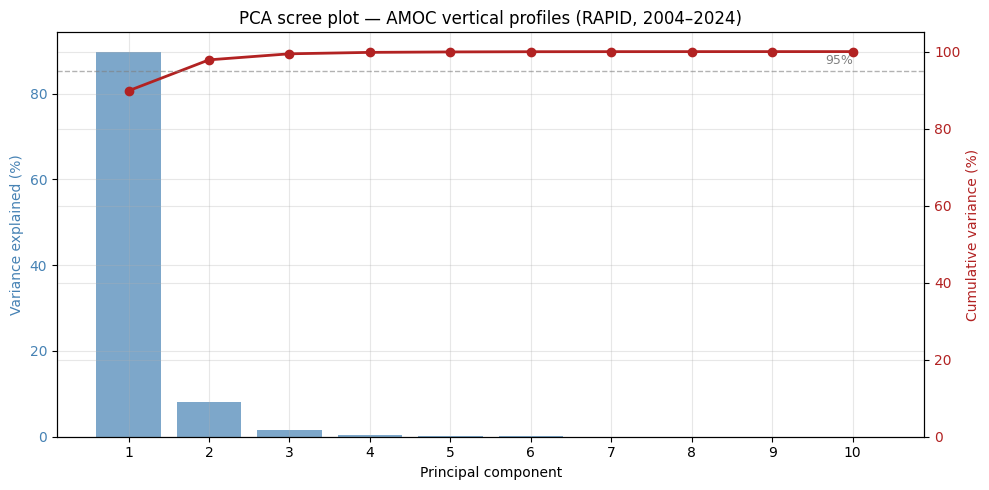
\includegraphics[width=0.8\textwidth]{figures/data_pipeline/pca_scree.png}
    \caption[Variance explained by the vertical PCA modes.]{\textbf{The vertical
    variability of the AMOC is almost one-dimensional.} Variance explained by each
    principal component of the 307-level vertical profiles. The first mode alone
    explains \SI{89.82}{\percent} and the first two together \SI{97.86}{\percent};
    the sharp elbow after the second mode marks where structure gives way to noise.
    This is the two-coordinate latent space the experiential representation is
    built on.}
    \label{fig:pca-scree}
\end{figure}

 
Both modes have a clear physical meaning and this is important because they provide a tangible interpretation of the abstract components. The first mode, PC1, has the same sign at every depth and peaks near 1150~m, close to the depth at which the average profile itself peaks (\S\ref{subsec:scene-column}). When its value rises, the whole overturning cell grows stronger while keeping its shape; when it falls, the cell weakens as a whole. PC1 is the \emph{intensity} of the circulation, and it is close to ninety per cent of what the AMOC does from one day to the next. The second mode, PC2, changes sign once as it goes down through the water column: it strengthens the cell at one depth while weakening it at another. It is the \emph{vertical redistribution} of the circulation --- a smaller but genuine shift in the shape of the overturning around its mean.

% figures/detect/fig_mode_shapes.tex — loads PDF exported from NB03
% Requires \usepackage{graphicx}. Export the PC1 & PC2 loading profiles
% (Sv-scaled: components·√λ, i.e. eof1/eof2) as
% figures/detect/mode_shapes.pdf.
\begin{figure}[!ht]
    \centering
    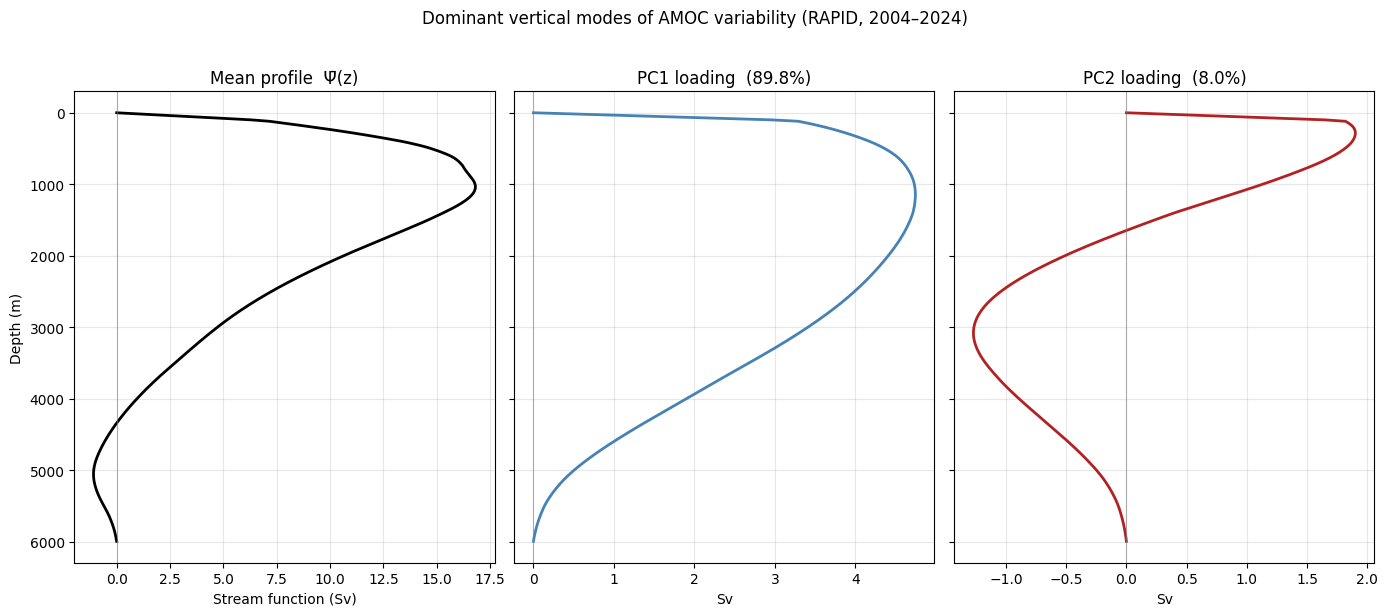
\includegraphics[width=1\textwidth]{figures/data_pipeline/mode_shapes.png}
    \caption[The two vertical modes: intensity and redistribution.]{\textbf{The
    two modes that explain the AMOC's vertical anatomy.} Each curve is a loading
    profile plotted against depth. PC1 (intensity) is a \emph{monopole}: the same
    sign at every depth, peaking near 1150~m where the mean profile peaks, so a
    change in its score strengthens or weakens the whole overturning cell coherently.
    PC2 (redistribution) is a \emph{dipole}: it changes sign once with depth,
    strengthening the cell at one level while weakening it at another. Loadings are
    Sv-scaled for display. Together these two shapes carry \SI{97.86}{\percent} of
    the vertical variability.}
    \label{fig:mode-shapes}
\end{figure}
 
This is where the analysis first touches the thesis directly. It would be easy to assign meanings to these modes after the fact; that is not what happens here. The intensity mode is recovered from the data and then confirmed against a known event, which is a stronger position to argue from. Followed through time, PC1 drops sharply during 2009--2010 --- the most thoroughly documented weakening in the observational record --- reaching a period mean PC1 score of $-23.97$ against a whole-record mean of zero.\footnote{The same 2009--2010 event shows up independently in the raw depth--time field, in this intensity series, and later in the anomaly detector: three methods, one physical episode.} That a single line can still carry an event first seen in the full depth--time field is a small but real proof of the thesis claim --- that this system can be re-represented in fewer dimensions without losing what matters. The PC1--PC2 plane, holding \SI{97.86}{\percent} of the vertical anatomy in just two coordinates, is the latent space along which the profiles will breathe faithfully through time in the experiential condition of Chapter~\ref{ch:translate}.

% -------------------------------------------------------------------------
\section{An Essentially Flat Manifold Geometry}
\label{sec:detect-ae}
 
Since PCA is a linear method, an important question is whether a linear representation is sufficient to capture the structure of the AMOC data: if the underlying geometry were strongly non-linear, a linear projection could oversimplify it and lose information. The comparison that follows is interpretable because of a known result: an autoencoder with linear activations recovers the same subspace as PCA, so any advantage a non-linear autoencoder shows at equal dimensionality is attributable to curvature in the data manifold \citep{baldi1989}. A near-zero gap is therefore evidence of flatness, not merely of a tie. The second objective (O1.2) therefore tests this assumption by comparing PCA with a non-linear autoencoder trained on the same 14{,}596 AMOC profiles. Both models are evaluated using the same number of latent dimensions. If the latent structure were genuinely non-linear, the autoencoder would be expected to reconstruct the data more accurately. If not, PCA should perform equally well.
 
The results clearly support the latter interpretation. Across latent dimensions from one to five, the non-linear autoencoder never outperformed PCA. Instead, PCA consistently achieved slightly better reconstruction accuracy, with differences ranging from $-0.06$ to $-0.15$ percentage points in its favour (Table~\ref{tab:ae-gap}). At the two-dimensional representation used throughout this thesis, PCA reconstructed \SI{97.86}{\percent} of the variance, compared with \SI{97.77}{\percent} for the autoencoder, a difference of less than one tenth of a percentage point.\footnote{The surface and seafloor levels were excluded from the autoencoder input because the streamfunction is fixed to zero at both boundaries by mass conservation and therefore contains no learnable variance.} These findings confirm H2. Even when given the flexibility to learn complex non-linear transformations, the autoencoder found no meaningful structure beyond that already captured by the linear PCA representation.

% figures/data_pipeline/tab_ae_gap.tex — autoencoder vs PCA at matched latent dimension
% Numbers verified against NB05. Requires \usepackage{booktabs}.
\begin{table}[!ht]
    \centering
    \small
    \caption[Autoencoder versus PCA at matched latent dimension.]{Reconstruction
    of the vertical profiles by a non-linear autoencoder against linear PCA, at
    matched latent dimension $k$. The gap is negative at every $k$: PCA is never
    beaten, so the manifold is flat.}
    \label{tab:ae-gap}
    \begin{tabular}{@{}crrr@{}}
        \toprule
        \textbf{$k$} & \textbf{PCA cum.\ \%} & \textbf{AE $R^2_{\mathrm{Sv}}$ \%} & \textbf{Gap (pp)} \\
        \midrule
        1 & 89.82 & 89.67 & $-0.15$ \\
        2 & 97.86 & 97.77 & $-0.08$ \\
        3 & 99.42 & 99.36 & $-0.06$ \\
        4 & 99.80 & 99.74 & $-0.06$ \\
        5 & 99.91 & 99.83 & $-0.08$ \\
        \bottomrule
    \end{tabular}
\end{table}

% figures/detect/fig_manifold.tex — loads PDF exported from NB03/NB05
% Requires \usepackage{graphicx}. Export the PC1-PC2 latent cloud
% (and/or the AE-vs-PCA comparison) as figures/detect/manifold.pdf.
\begin{figure}[!ht]
    \centering
    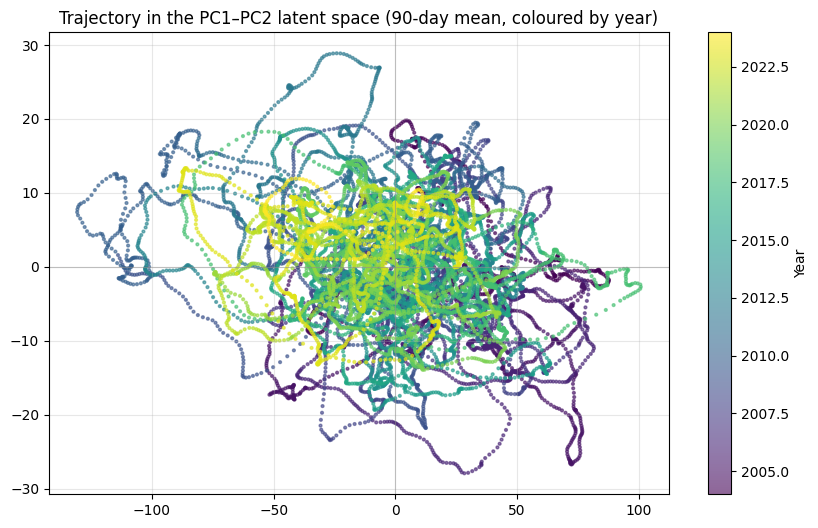
\includegraphics[width=0.85\textwidth]{figures/data_pipeline/fig_manifold.png}
    \caption[The flat latent manifold of AMOC profiles.]{\textbf{The manifold of
    AMOC vertical profiles is flat.} Each point is one day, placed by its two
    latent coordinates --- PC1 (intensity) and PC2 (vertical redistribution). A
    non-linear autoencoder trained on the same profiles reconstructs them no
    better than linear PCA at any latent dimension (gap $-0.06$ to $-0.15$
    percentage points; see Table~\ref{tab:ae-gap}), confirming that two straight
    coordinates capture the structure without distortion.}
    \label{fig:manifold}
\end{figure}


This result is important because it justifies the use of the latent coordinates throughout the \emph{Translate} phase of the thesis. If the underlying manifold had been strongly curved, representing the system using the first two principal components would have introduced distortions by forcing a non-linear structure into a linear space. Instead, the results show that the latent manifold is effectively linear. As a consequence, the first two principal components provide a representation that is both highly interpretable and highly faithful to the original data. The coordinates can therefore be meaningfully interpreted as distinct modes of AMOC variability without sacrificing representational accuracy. In this case, interpretability comes at virtually no cost in fidelity, making the proposed representation both scientifically defensible and suitable as the basis for the experiential visualisations developed in the following chapter.

% -------------------------------------------------------------------------
\section{Early Warning Signals \& Null Result}
\label{sec:detect-ews}
 
The third objective (O1.3) investigates whether the record contains early warning signs of an approaching tipping point. According to the theory of critical slowing down, a system approaching a bifurcation is expected to show increasing variance and increasing lag-1 autocorrelation \citep{dakos2012, scheffer2009}. Testing this hypothesis requires particular care, and this is where the analysis highlights an important methodological issue.

At first glance the results appear very strong. The rolling variance of the intensity series trends upward, with Kendall's $\tau = +0.078$ and a p-value of $2\times10^{-42}$; the rolling autocorrelation likewise increases, with $\tau = +0.088$ and a p-value of $1\times10^{-52}$. Taken at face value these would be an extremely strong signal. The interpretation is misleading, because the rolling windows overlap substantially and the thousands of calculated values are not independent observations.\footnote{Kendall's test assumes independence. Here the rolling statistics use heavily overlapping 730-day windows, so consecutive values are highly dependent --- an effect amplified by the strong autocorrelation of the original series ($0.943$). The software returns a very small p-value without accounting for that dependence, making the result appear more certain than it is.} When the effective number of independent observations is used instead --- approximately 19.5 non-overlapping 730-day windows --- and the test is corrected accordingly, the apparent trends disappear. The corrected p-value for the variance trend is \textbf{0.634}, while for the autocorrelation trend it is \textbf{0.595}. Neither result is statistically significant (Table~\ref{tab:ews}). The initial strong signal was therefore caused by treating dependent observations as if they were independent.

% figures/data_pipeline/tab_ews.tex — early-warning trends, naive vs corrected significance
% Numbers verified against NB04. Requires \usepackage{booktabs}.
\begin{table}[!ht]
    \centering
    \small
    \caption[Early-warning trends: naive versus corrected significance.]{Kendall's
    $\tau$ trend tests for the two classical early-warning signals. The naive
    p-values treat overlapping windows as independent; the corrected p-values
    count the $\sim$19.5 independent windows the record contains. Neither trend is
    significant.}
    \label{tab:ews}
    \begin{tabular}{@{}lcccc@{}}
        \toprule
        \textbf{Signal} & \textbf{Kendall $\tau$} & \textbf{Naive p} & \textbf{Corrected p} & \textbf{Verdict} \\
        \midrule
        Rolling variance & $+0.078$ & $2\times10^{-42}$ & 0.634 & not significant \\
        Rolling AR(1)     & $+0.088$ & $1\times10^{-52}$ & 0.595 & not significant \\
        \bottomrule
    \end{tabular}
\end{table}

% figures/detect/fig_ews.tex — loads PDF exported from NB04
% Requires \usepackage{graphicx}. Export the rolling variance / AR1 panels
% as figures/detect/ews.pdf.
\begin{figure}[!ht]
    \centering
    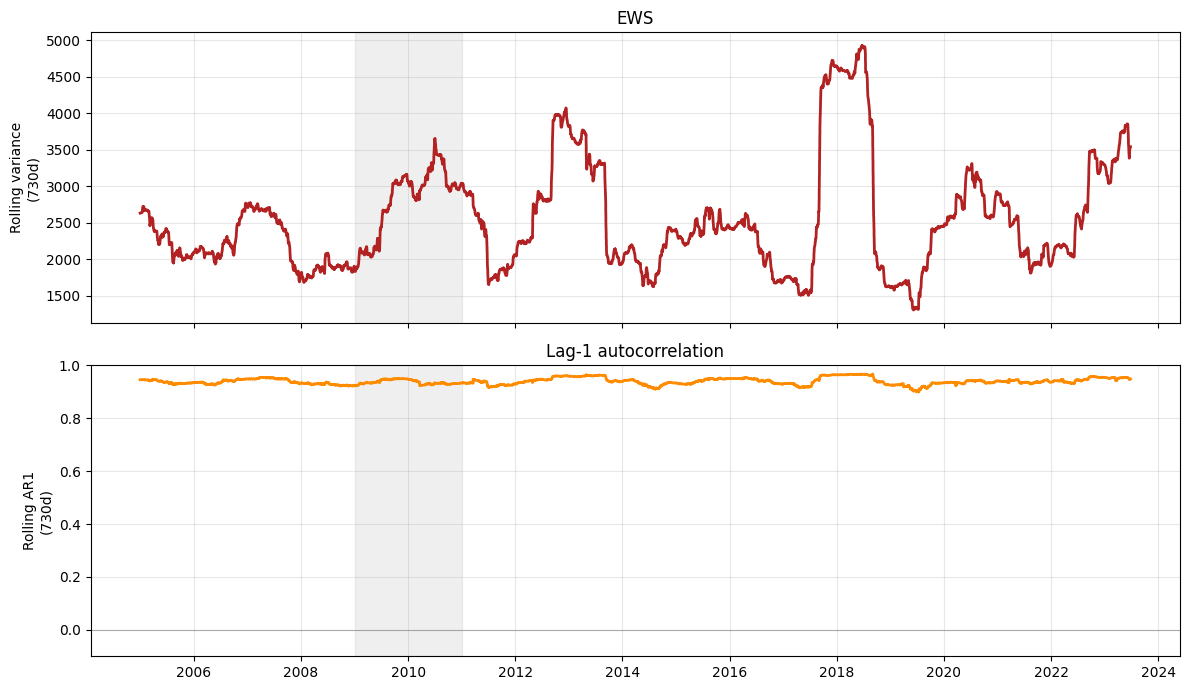
\includegraphics[width=0.9\textwidth]{figures/data_pipeline/ews.png}
    \caption[Early warning signals: rolling variance and autocorrelation.]{\textbf{No
    rigorous early-warning trend.} Rolling variance and lag-1 autocorrelation of the
    intensity series over the record. Both oscillate without a sustained climb.
    Their naive trend p-values ($\sim$$10^{-42}$) are artefacts of heavily
    overlapping windows; corrected for the $\sim$19.5 independent windows the
    record actually contains, the trends are not significant (p~$=$~0.634 and
    0.595; Table~\ref{tab:ews}).}
    \label{fig:ews}
\end{figure}


The final conclusion is therefore a \emph{null result}. Once the dependence structure of the data is properly considered, the classical early-warning indicators cannot be distinguished from noise. This supports H3 in its null form and represents an important methodological contribution rather than a limitation. A positive result obtained by interpreting the statistics incorrectly would have been more appealing, but it would not have been reliable. Demonstrating that an apparently strong signal disappears once statistical dependence is addressed is the substantive result here. The boundary between pattern detection and prediction that this phase observes is recorded in Appendix~\ref{app:limits-detect}.

% -------------------------------------------------------------------------
\section{Anomaly Detection}
\label{sec:detect-anomalies}

Early-warning analysis looks for slow \emph{trends}. A different question is about individual \emph{events}: which moments depart from the normal behaviour of the system. An Isolation Forest applied to the PC1--PC2 coordinates identifies \SI{5}{\percent} of the record, corresponding to 730 profiles, as anomalous. Looking at when these fall reveals an important pattern: they are concentrated in 2009--2010 (158 profiles), 2012--2013 (100 profiles) and 2018 (66 profiles). However, the anomaly score does not increase over time. The unusual moments are distributed across the record rather than accumulating toward the end, providing another indication that the system is not showing a progressive movement toward a threshold.

% figures/detect/fig_anomalies.tex — loads PDF exported from NB04
% Requires \usepackage{graphicx}. Export the anomaly scatter / timeline
% as figures/detect/anomalies.pdf.
\begin{figure}[!ht]
    \centering
    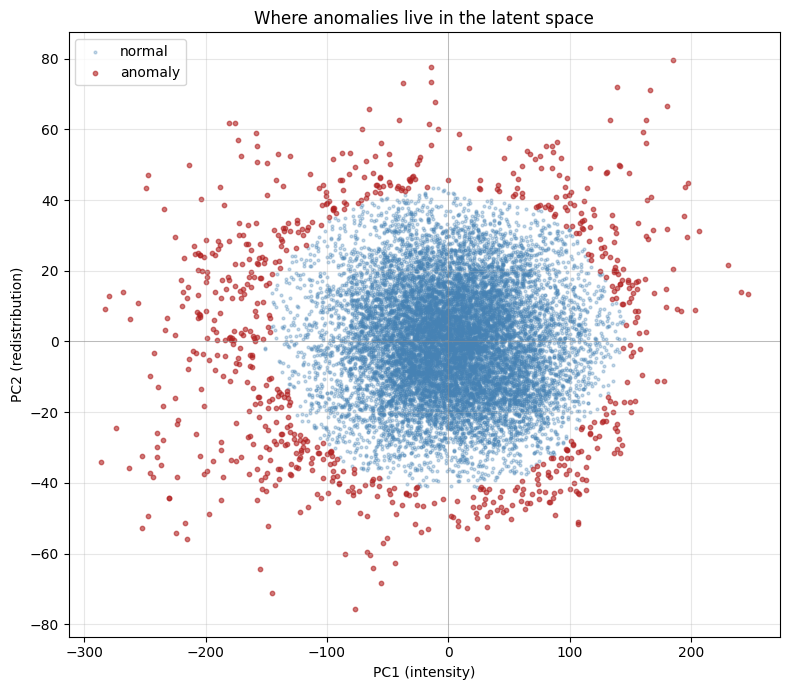
\includegraphics[width=0.9\textwidth]{figures/data_pipeline/anomalies.png}
    \caption[Isolation Forest anomalies across the record.]{\textbf{Discrete
    anomalous events, spread across the record.} The Isolation Forest flags
    \SI{5}{\percent} of days (730) as anomalous in the PC1--PC2 plane. They cluster
    in 2009--2010 (158 days), 2012--2013 (100) and 2018 (66), with no trend over
    time --- corroborating the early-warning null from a different method. These
    moments become perceptible texture (grammar principle~P3) in
    Chapter~\ref{ch:translate}.}
    \label{fig:anomalies}
\end{figure}


Two aspects are important for this thesis. First, this analysis supports the null result from a completely independent perspective: an algorithm that does not rely on early-warning theory also finds no gradual shift, but rather isolated events distributed across the twenty-year record. It reaches the same conclusion through a different method.\footnote{The anomaly clusters correspond to independently identified features --- the 2009--2010 weakening and the variance peaks of 2012--2013 and 2018 --- with \SI{41.4}{\percent} of anomalous profiles falling in the highest quarter of local variance. Different methods reveal the same physical behaviour.} Second, these anomalies provide the basis for a specific design decision. Following the grammar introduced in Chapter~\ref{ch:literature}, departures from the normal regime can be translated into local changes in perceptual texture (principle~P3). The moments identified by the detector are therefore the same moments that the experiential representation will transform into perceptible changes --- meaning that anomaly detection is not only a result about the AMOC, but also a direct input for how the AMOC is represented.

% -------------------------------------------------------------------------
\section{Observation Against Reanalysis}
\label{sec:detect-copernicus}

The final step compares the RAPID observations with the Copernicus GREP reanalysis ensemble over the 237 months they share, to characterise how well the reanalysis reproduces the observed signal and to identify the uncertainty the \emph{translate} phase must communicate. Agreement is moderate: correlation 0.754, a small bias of $+0.584$~Sv with RAPID slightly stronger, and a root-mean-square difference of 2.300~Sv. Both remain close to 17~Sv and vary similarly over time, so the reanalysis captures the overall behaviour of the circulation even where it misses individual months.

The most informative result concerns uncertainty coverage. RAPID falls within the reanalysis ensemble's own $\pm1$ standard-deviation range in only \SI{40.1}{\percent} of months.\footnote{If the ensemble spread represented a well-calibrated estimate of its own uncertainty, the observation should fall within the one-standard-deviation range much more often. A lower coverage indicates that the spread is too narrow compared with the actual errors.} A model ensemble with a realistic uncertainty range should capture the observation more frequently. This low coverage indicates that the ensemble is \emph{overconfident}: its reported uncertainty is smaller than the real error. This point is important for the thesis because the ensemble spread is exactly what the \emph{translate} phase converts into perceptible uncertainty, following design-grammar principle~P4. Understanding that this uncertainty is underestimated is therefore part of representing it honestly: the visualisation can communicate the model's uncertainty while making clear that the real uncertainty is likely larger.

% -------------------------------------------------------------------------
\section{Analytical Summary}
\label{sec:detect-summary}

The analytical phase hands the \emph{translate} phase a documented substrate rather than an assumed one. Two interpretable coordinates --- intensity and vertical redistribution --- carry \SI{97.86}{\percent} of the AMOC's vertical variability, and a non-linear model confirms the manifold is flat enough that using them introduces no relevant distortion. The record shows no robust early-warning trend but does contain discrete anomalies that can become perceptual texture, and the comparison with the reanalysis yields an uncertainty estimate that is physically meaningful although too narrow. Each of these is a justified input for what follows: a compact, faithful, interpretable, event-aware and uncertainty-carrying substrate on which an invisible system can be made perceptible without being misrepresented.